\section{Конструкторский раздел \hfill}
\vspace{\baselineskip}

\subsection{Разработка алгоритмов}

На рисунках  \ref{fig:diagram-standard}, \ref{fig:diagram-vinograd} и \ref{fig:diagram-vinograd-opt} представлены схемы стандартного алгоритма, алгоритма Винограда и алгоритма Винограда с оптимизациями соответственно.

На схеме на рисунке \ref{fig:diagram-vinograd} видно, что для алгоритма Винограда худшим случаем являются матрицы с нечётным размером, а лучшим -- с чётным, так как в этой ситуации отпадает необходимость в последнем цикле.

Будем использовать следующие оптимизации алгоритма Винограда:
\begin{enumerate}
    \item замену операции $x = x + k$ на $x += k$;
    \item замену умножения на 2 на побитовый сдвиг;
    \item предвычисление слагаемых для алгоритма.
\end{enumerate}
\newpage

\begin{figure}[h!btp]
	\centering
	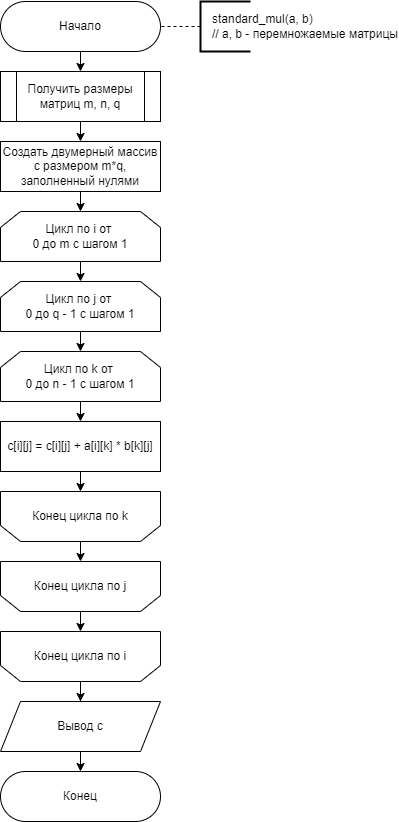
\includegraphics[width=250pt]{inc/diagram-standard.png}
	\caption{Схема стандартного алгоритма умножения матриц}
	\label{fig:diagram-standard}	
\end{figure}
\clearpage

\begin{figure}[h!btp]
	\centering
	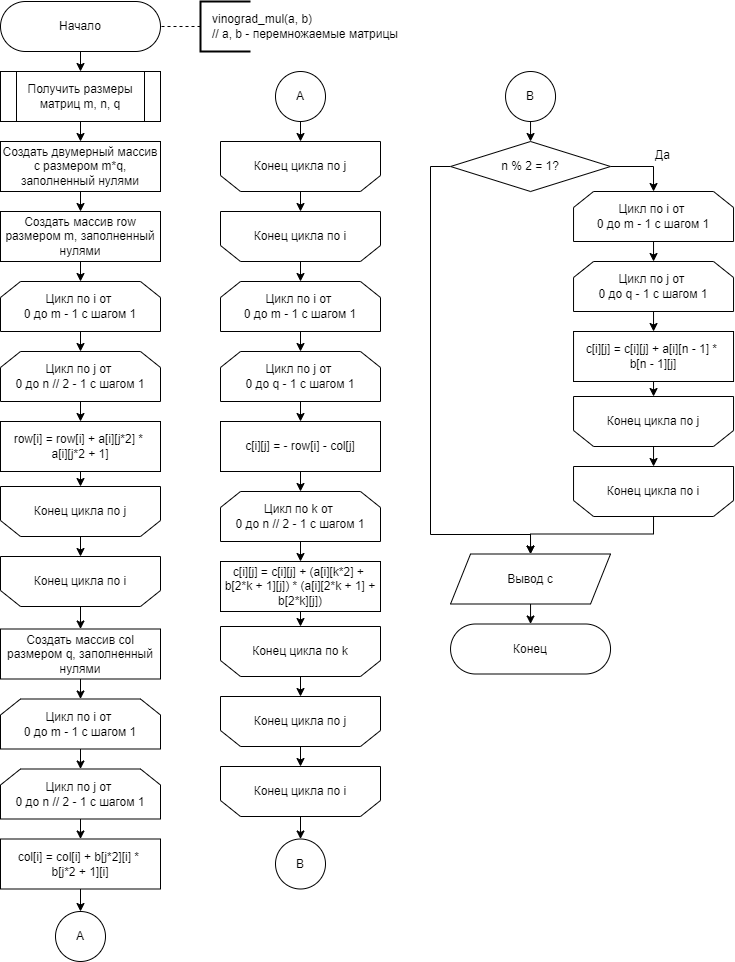
\includegraphics[width=450pt]{inc/diagram-vinograd.png}
	\caption{Схема алгоритма Винограда умножения матриц}
	\label{fig:diagram-vinograd}	
\end{figure}
\clearpage

\begin{figure}[h!btp]
	\centering
	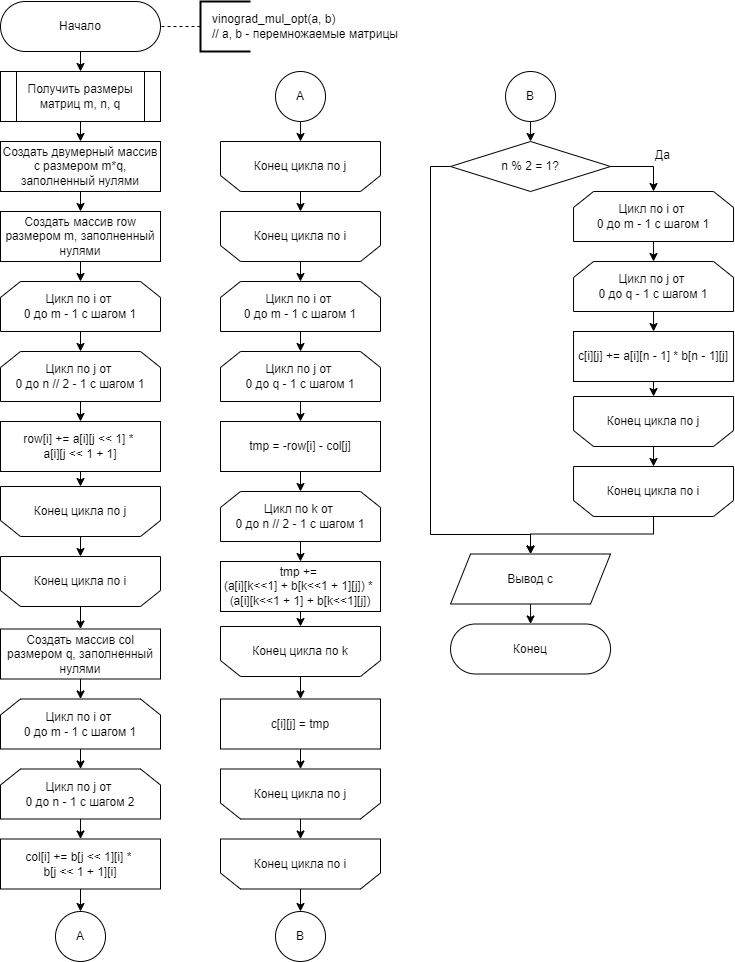
\includegraphics[width=450pt]{inc/diagram-vinograd-opt.png}
	\caption{Схема оптимизированного алгоритма Винограда}
	\label{fig:diagram-vinograd-opt}	
\end{figure}
\clearpage

\subsection{Оценка трудоемкости}

Для последующего вычисления трудоемкости необходимо ввести модель вычислений.

\begin{enumerate}

	\item Трудоемкость следующих базовых операций единична:
	+, -, =, +=, -=, ==, !=, <, >, <=, >=, [], ++, --, <<, >>.
	
	Операции *, \%, / имеют трудоемкость 2.
	
	\item Трудоемкость цикла for(k = 0; k < N; k++) \{тело цикла\} рассчитывается как:
	\begin{equation}
		\label{for:for}
		f_{for} = f_{\text{инициал.}} + f_{\text{сравн.}} + N(f_{\text{тела}} + f_{\text{инкр.}} + f_{\text{сравн.}})
	\end{equation}
	
	\item Трудоемкость условного оператора \code{if (условие) then A else B} рассчитывается как:
	
	\begin{equation}
		\label{for:if}
		f_{if} = f_{\text{условия}} +
		\begin{cases}
			min(f_A, f_B), & \text{л.с.}\\
			max(f_A, f_B), & \text{х.с.}
		\end{cases}
	\end{equation}
	
\end{enumerate}


Произведем теоретическую оценку трудоемкости алгоритмов умножения матриц.

\begin{enumerate}
	\item Трудоемкость стандартного алгоритма рассчитывается по формуле
	\begin{equation}
	    \label{f_s}
		f=2+m(4+q(4+14n))=14mnq+4mq+4m+2
	\end{equation}

	\item Трудоемкость базового алгоритма Винограда рассчитывается по формуле (\ref{f_v}), представляющей собой сумму трудоемкостей четырех циклов (формулы \ref{f1_v} -- \ref{f4_v}).
	
	\begin{equation}
	    \label{f1_v}
		f1=2+m(2+4+\frac{n}{2}\cdot19)=\frac{19}{2}mn+6m+2
	\end{equation}
	
	\begin{equation}
		f2=2+q(6+\frac{n}{2}\cdot19)=\frac{19}{2}qn+6q+2
	\end{equation}
	
	\begin{equation}
		f3=2+m(4+q(13+\frac{n}{2}\cdot32))=16mnq+13mq+4m+2
	\end{equation}
	
	\begin{equation}
	    \label{f4_v}
		f4=3+
	    \begin{cases}
		    $$0$$, & \text{л.с.}\\
		    $$2+m(4+16q)=16mq+4m+2$$, & \text{х.с.}
	    \end{cases}
	\end{equation}
	
	\begin{equation}\begin{split}
	    \label{f_v}
		f = 16mnq&+13mq+\frac{19}{2} mn+\frac{19}{2} qn+6m+6q+6+ \\
        &+\begin{cases}
	        $$0$$, & \text{л.с.}\\
	        $$16mq+4m+2$$, & \text{х.с.}
        \end{cases}
	\end{split}\end{equation}

	\item Трудоемкость оптимизированного алгоритма Винограда рассчитывается по формуле \ref{f_ov}, представляющей собой сумму трудоемкостей четырех циклов (формулы \ref{f1_ov} -- \ref{f4_ov}).
	
	\begin{equation}
	    \label{f1_ov}
		f1=2+m(6+\frac{n}{2}\cdot15)=\frac{15}{2}mn+6m+2
	\end{equation}
	
	\begin{equation}
		f2=2+q(6+\frac{n}{2}\cdot15)=\frac{15}{2}qn+6q+2
	\end{equation}
	
	\begin{equation}
		f3=2+m(4+q(11+\frac{n}{2}\cdot18+3))=9mnq+14mq+7m+2
	\end{equation}
	
	\begin{equation}
	    \label{f4_ov}
		f4=3+
	    \begin{cases}
		    $$0$$, & \text{л.с.}\\
		    $$2+m(4+13q)=13mq+4m+2$$, & \text{х.с.}
	    \end{cases}
	\end{equation}
	
	\begin{equation}\begin{split}
	    \label{f_ov}
		f=9mnq&+14mq+\frac{15}{2} mn+\frac{15}{2} qn+6m+6q+6+ \\
        &+\begin{cases}
	        $$0$$, & \text{л.с.}\\
	        $$13mq+4m+2$$, & \text{х.с.}
        \end{cases}
	\end{split}\end{equation}
\end{enumerate}

Лучший случай алгоритма Винограда и оптимизированного алгоритма Винограда --- четная размерность $n$ матрицы, т.к. в этом случае не производится заход в последний цикл.

\subsection*{Вывод}

Были разработаны схемы алгоритмов, позволяющих с помощью различных подходов находить произведение матриц, а также была дана оценка трудоемкости для рассмотренных алгоритмов.
